\documentclass[12pt, a4paper]{article}

% --- Cấu hình gói ngôn ngữ và font ---
\usepackage[utf8]{inputenc}
\usepackage[vietnamese]{babel}
\usepackage{amsmath, amssymb, amsfonts, amsthm}
\usepackage{geometry}
\geometry{left=2.5cm, right=2.5cm, top=2.5cm, bottom=2.5cm}
\usepackage{graphicx}
\usepackage{hyperref}
\usepackage{algorithm}
\usepackage{algorithmic}
\usepackage{booktabs}
\usepackage{bm}
\usepackage{parskip}
\usepackage{float}

% --- Cấu hình liên kết ---
\hypersetup{
	colorlinks=true,
	linkcolor=blue,
	urlcolor=cyan,
	citecolor=red,
}

% --- Lệnh toán học ---
\newcommand{\E}{\mathbb{E}}
\newcommand{\R}{\mathbb{R}}
\DeclareMathOperator{\Tr}{tr}

% --- THÔNG TIN ---
\title{\textbf{BÁO CÁO CHUYÊN ĐỀ}\\
	\LARGE \textbf{NATURAL EVOLUTION STRATEGIES (NES)}\\
	\large Phương pháp Tiến hóa dựa trên Gradient Tự nhiên cho Tối ưu hóa Hộp đen}

\author{
	\textbf{Nhóm thực hiện:}\\
	Lê Thiên Quân -- 24520027\\
	Đinh Mạnh Hùng -- 24520014
}

\date{\today}

\begin{document}
	
	% --- TRANG BÌA ---
	% ====================== TRANG BÌA ======================
	\begin{titlepage}
		\centering
		% -------- Trường / Khoa --------
		{\textbf{ĐẠI HỌC QUỐC GIA TP. HỒ CHÍ MINH}}\\[0.2cm]
		{\Large \textbf{TRƯỜNG ĐẠI HỌC CÔNG NGHỆ THÔNG TIN}}\\[0.15cm]
		{\large \textbf{KHOA KHOA HỌC MÁY TÍNH}}
		
		\vspace{1cm}
		
		
\includegraphics[width=0.22\textwidth]{logo_uit.jpg}\\[1.2cm]
		
		\vspace{1.5cm}
		
		% -------- Loại báo cáo --------
		{\large \textbf{BÁO CÁO ĐỒ ÁN}}
		
		\vspace{1cm}
		
		% -------- Tiêu đề chính --------
		{\Huge \bfseries
			NATURAL EVOLUTION
		}
		
		{\Huge \bfseries
			STRATEGIES
		}
		
		\vspace{0.6cm} % <<< GIẢI QUYẾT VẤN ĐỀ "DÍNH CHỮ"
		
		{\Large \bfseries
			Chiến lược Tiến hóa Tự nhiên
		}
		
		\vspace{2.5cm}
		
		\vspace{1.5cm}
		
		% -------- Thông tin --------
		\begin{tabular}{@{}l@{}}
			\textbf{Giảng viên hướng dẫn: TS. Lương Ngọc Hoàng} \dotfill \\[0.6cm]
			\textbf{Nhóm thực hiện:} \\[0.2cm]
			Lê Thiên Quân -- 24520027 \\[0.15cm]
			Đinh Mạnh Hùng -- 24520014
		\end{tabular}
		
		\vfill
		
		% -------- Địa điểm & thời gian --------
		TP. Hồ Chí Minh, \today
		
	\end{titlepage}
	% ======================================================
	
	
	
	\tableofcontents
	\newpage
	
	% =========================================================
	\begin{abstract}
		Natural Evolution Strategies (NES) là một lớp thuật toán tối ưu hóa hộp đen dựa trên việc tối ưu hóa trực tiếp các tham số của phân phối tìm kiếm. Khác với các phương pháp tiến hóa truyền thống vốn phụ thuộc nhiều vào heuristic, NES được xây dựng trên nền tảng toán học chặt chẽ của \emph{Natural Gradient} và hình học thông tin.  
		
		Báo cáo này trình bày cơ sở lý thuyết của NES, phân tích nguyên nhân khiến Gradient thông thường trở nên mất ổn định khi áp dụng cho phân phối Gaussian, và giới thiệu biến thể \textbf{xNES (Exponential NES)} nhằm khắc phục các hạn chế về tính ổn định số và chi phí tính toán. Các thực nghiệm trên hàm Rastrigin cho thấy xNES đạt khả năng hội tụ ổn định và hiệu quả, tương đương với các phương pháp hiện đại như CMA-ES.
	\end{abstract}
	
	% =========================================================
	\section{Giới thiệu}
	
	\subsection{Tối ưu hóa Hộp đen}
	Trong nhiều bài toán thực tế như điều khiển robot, tối ưu siêu tham số hay thiết kế kỹ thuật, hàm mục tiêu $f(x)$ không có biểu thức giải tích rõ ràng. Các bài toán này chỉ cho phép truy cập thông qua việc đánh giá giá trị hàm tại các điểm thử nghiệm và thường được gọi là \textbf{bài toán tối ưu hóa hộp đen}.  
	
	Đặc trưng của lớp bài toán này bao gồm:
	\begin{itemize}
		\item Không có thông tin đạo hàm bậc nhất hoặc bậc hai.
		\item Hàm mục tiêu có thể nhiễu và không trơn.
		\item Chi phí đánh giá hàm thường rất cao.
	\end{itemize}
	
	Do đó, các phương pháp tối ưu cổ điển dựa trên gradient không còn phù hợp.
	
	\subsection{Động lực phát triển Natural Evolution Strategies}
	Các thuật toán tiến hóa (Evolutionary Algorithms) là một hướng tiếp cận phổ biến cho tối ưu hóa hộp đen. Trong số đó, \textbf{Evolution Strategies (ES)} với đại diện tiêu biểu là \textbf{CMA-ES} đạt hiệu năng rất cao. Tuy nhiên, CMA-ES dựa trên nhiều heuristic phức tạp, gây khó khăn cho việc phân tích lý thuyết.
	
	Natural Evolution Strategies được đề xuất nhằm:
	\begin{itemize}
		\item Cung cấp một khung tối ưu hóa dựa trên gradient có cơ sở toán học rõ ràng.
		\item Thực hiện cập nhật trực tiếp trên phân phối tìm kiếm.
		\item Đảm bảo tính bất biến theo tham số hóa.
	\end{itemize}
	
	% =========================================================
	\section{Cơ sở Toán học của NES}
	
	\subsection{Search Gradient}
	Thay vì tối ưu trực tiếp $f(x)$, NES tối ưu hóa kỳ vọng của hàm mục tiêu dưới phân phối tìm kiếm $\pi(z|\theta)$:
	\begin{equation}
		J(\theta) = \E_{z \sim \pi}[f(z)].
	\end{equation}
	
	Gradient của $J(\theta)$ có thể được viết lại bằng \textbf{log-likelihood trick}:
	\begin{equation}
		\nabla_\theta J = \E \left[ f(z)\nabla_\theta \log \pi(z|\theta) \right].
	\end{equation}
	
	Công thức này cho phép ước lượng gradient bằng phương pháp Monte Carlo, tạo nền tảng cho các thuật toán tiến hóa dựa trên gradient.
	
	\subsection{Vấn đề của Gradient thông thường}
	Xét phân phối Gaussian một chiều $\mathcal{N}(\mu,\sigma)$. Đạo hàm theo $\sigma$ có dạng:
	\begin{equation}
		\nabla_\sigma \log \pi(z) = \frac{(z-\mu)^2 - \sigma^2}{\sigma^3}.
	\end{equation}
	
	% ================== HÌNH DEMO GRADIENT EXPLOSION ==================
	% Demo sự bùng nổ gradient khi sigma tiến về 0
	% So sánh: Canonical ES / Vanilla Gradient
	% Gợi ý hình:
	%   - Biểu đồ sigma theo iteration
	%   - Hoặc trajectory bị bật khỏi optimum
	%
	\begin{figure}[H]
		     \centering
		     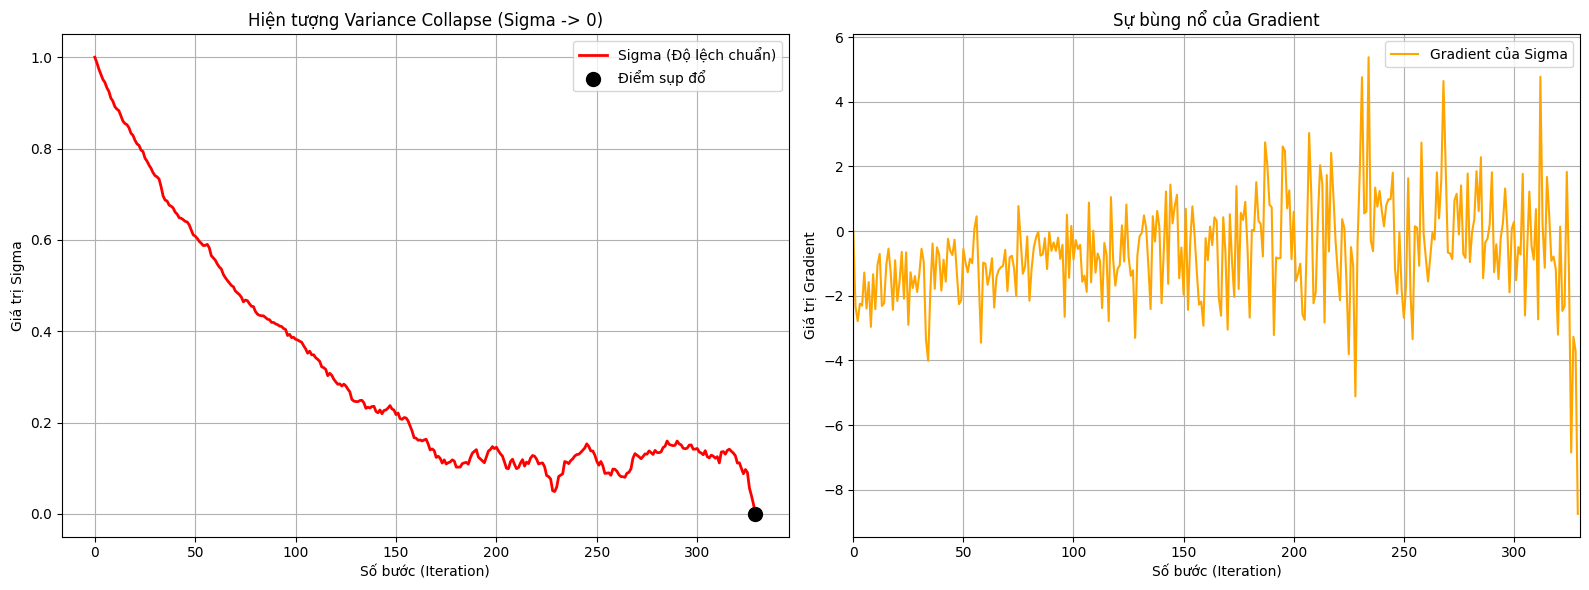
\includegraphics[width=0.9\textwidth]{BungNoGradient.png}
		     \caption{Hiện tượng bùng nổ gradient khi cập nhật trực tiếp theo $\sigma$}
	\end{figure}
	% ================================================================
	
	Khi thuật toán tiến dần đến nghiệm, $\sigma$ cần giảm để tăng độ chính xác. Tuy nhiên, khi $\sigma \to 0$, gradient trở nên không bị chặn, dẫn đến hiện tượng \textbf{bùng nổ gradient}. Điều này khiến thuật toán mất ổn định và không thể hội tụ.
	
	\subsection{Natural Gradient}
	Natural Gradient giải quyết vấn đề trên bằng cách đo khoảng cách trong không gian phân phối thông qua \textbf{Kullback–Leibler divergence}. Hướng cập nhật được xác định bởi:
	\begin{equation}
		\tilde{\nabla}_\theta J = F^{-1} \nabla_\theta J,
	\end{equation}
	trong đó $F$ là ma trận thông tin Fisher. Natural Gradient cho phép triệt tiêu ảnh hưởng của tham số hóa và đảm bảo bước cập nhật ổn định.
	
	% ================== HÌNH SO SÁNH GRADIENT ==================
	% Minh họa khác biệt giữa:
	% - Gradient thường (phụ thuộc tham số hóa)
	% - Natural Gradient (bất biến theo tham số)
	% Gợi ý hình: đường đi zig-zag vs đường đi thẳng
	%
	% ================== KHUNG HÌNH TIẾN HÓA (6 ẢNH) ==================
	% Minh họa đường đi / tiến hóa phân phối theo thời gian
	% Gợi ý iteration: 0, 10, 30, 50, 80, 120
	%
	\begin{figure}[H]
		\centering
		
		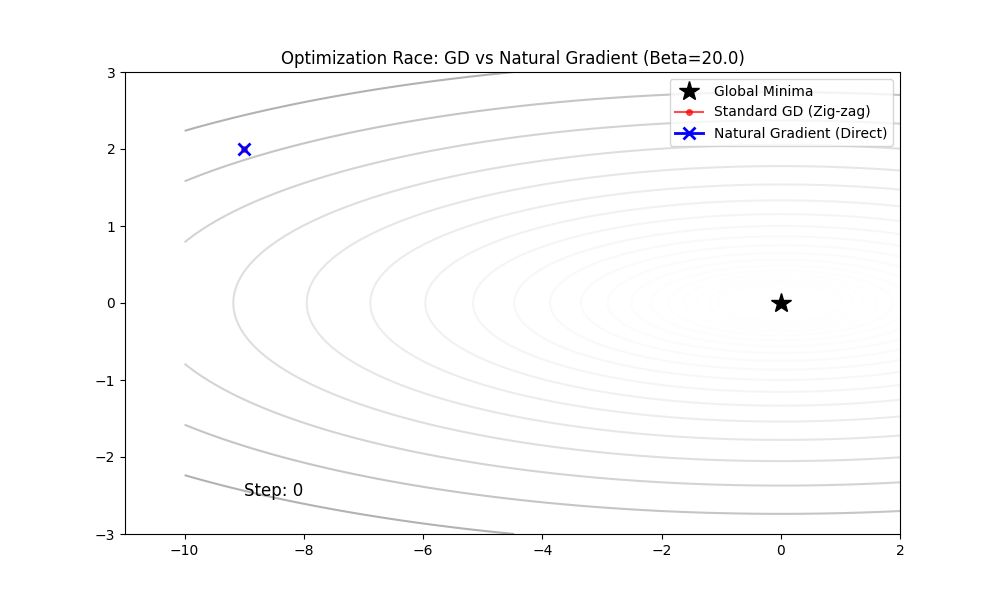
\includegraphics[width=0.32\textwidth]{BungNoGradient/frame_00_delay-0.16s.png}
		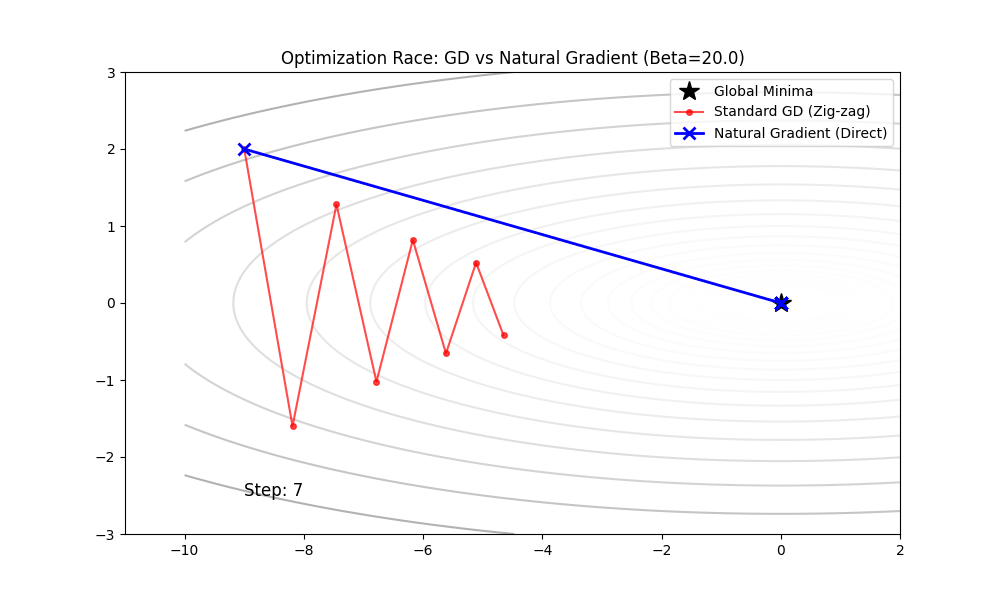
\includegraphics[width=0.32\textwidth]{BungNoGradient/frame_07_delay-0.16s.png}
		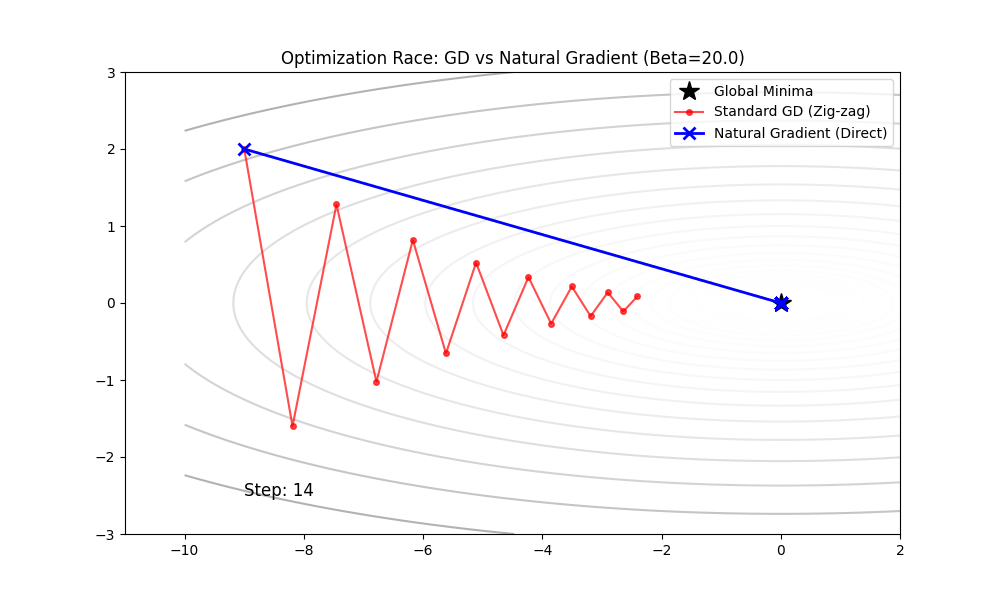
\includegraphics[width=0.32\textwidth]{BungNoGradient/frame_14_delay-0.16s.png}
		
		\vspace{0.3cm}
		
		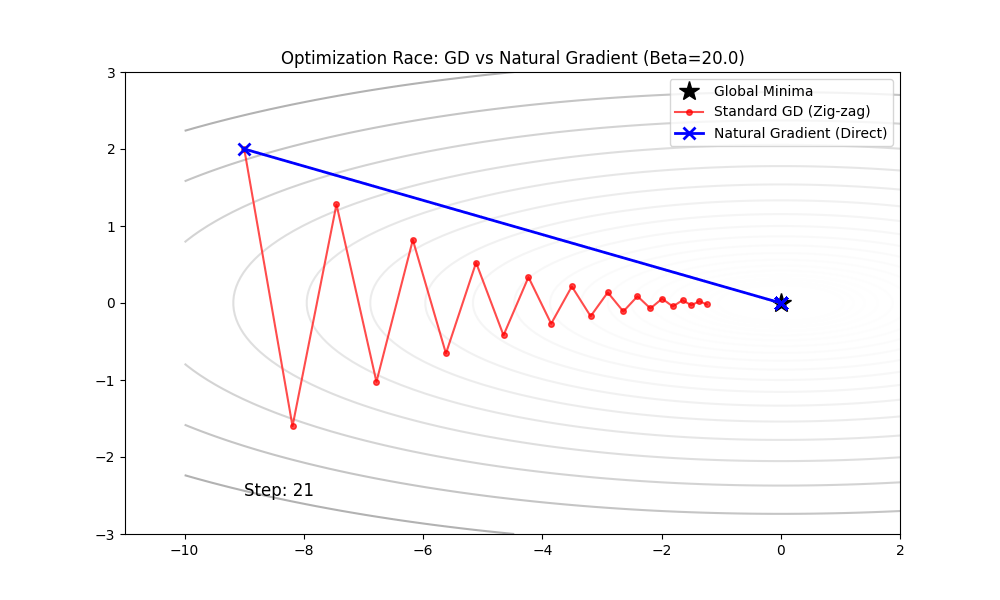
\includegraphics[width=0.32\textwidth]{BungNoGradient/frame_21_delay-0.16s.png}
		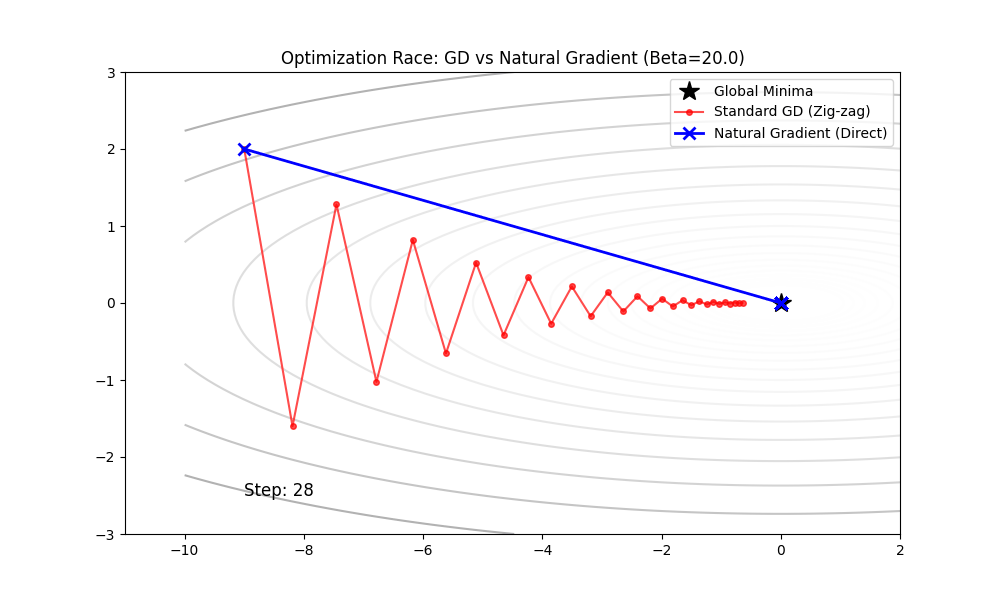
\includegraphics[width=0.32\textwidth]{BungNoGradient/frame_28_delay-0.16s.png}
		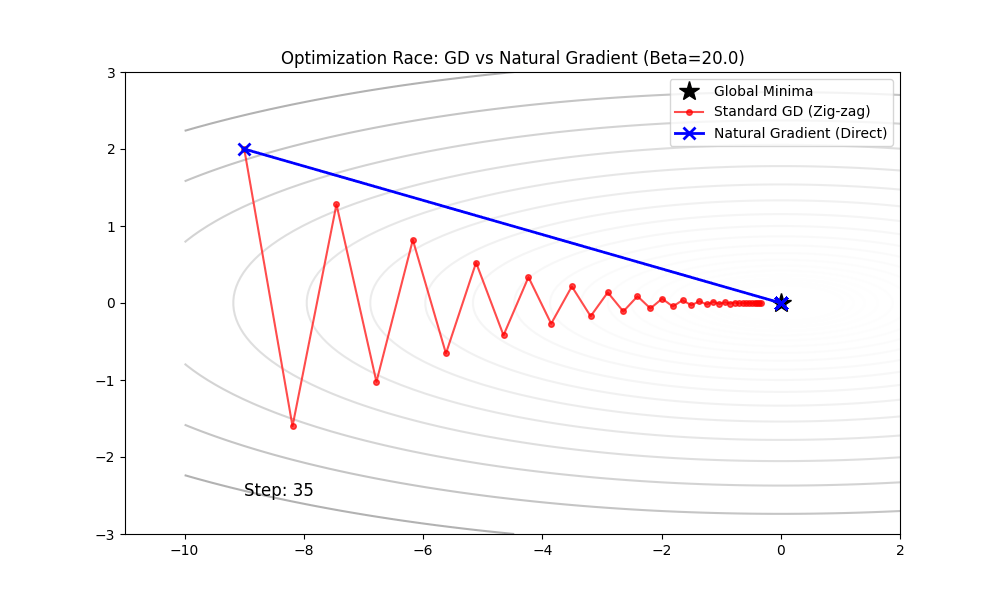
\includegraphics[width=0.32\textwidth]{BungNoGradient/frame_35_delay-0.16s.png}
		
		\caption{Sự khác nhau giữa Gradient thường và Natural Gradient}
		\label{fig:natural_gradient}
	\end{figure}
	% ================================================================
	
	% =========================================================
	\section{xNES -- Exponential Natural Evolution Strategies}
	
	\subsection{Hạn chế của Canonical NES}
	Mặc dù Natural Gradient cải thiện đáng kể độ ổn định, việc tính toán và nghịch đảo ma trận Fisher có độ phức tạp $O(d^3)$, không phù hợp với bài toán chiều cao. Ngoài ra, cập nhật cộng trực tiếp lên ma trận hiệp phương sai không đảm bảo tính xác định dương.
	
	\subsection{Ý tưởng chính của xNES}
	xNES khắc phục các hạn chế trên thông qua:
	\begin{itemize}
		\item \textbf{Tham số hóa mũ:} Cập nhật hiệp phương sai bằng ánh xạ mũ để đảm bảo tính xác định dương.
		\item \textbf{Hệ tọa độ tự nhiên:} Thực hiện cập nhật trong không gian nơi ma trận Fisher là đơn vị.
	\end{itemize}
	
	\subsection{Quy tắc cập nhật}
	Với $x_i = \mu + \sigma B z_i$, các gradient được xác định như:
	\[
	G_\delta = \sum u_i z_i, \quad
	G_M = \sum u_i (z_i z_i^\top - I).
	\]
	
	Cập nhật tham số:
	\begin{align}
		\mu &\leftarrow \mu + \eta_\mu \sigma B G_\delta,\\
		\sigma &\leftarrow \sigma \exp(\eta_\sigma G_\sigma /2),\\
		B &\leftarrow B \exp(\eta_B G_B /2).
	\end{align}
	
	\begin{algorithm}[H]
		\caption{xNES}
		\begin{algorithmic}[1]
			\STATE Initialize $\mu,\sigma,B$
			\LOOP
			\STATE Sample $z_i \sim \mathcal{N}(0,I)$
			\STATE Evaluate $f(x_i)$
			\STATE Compute gradients
			\STATE Update $\mu,\sigma,B$
			\ENDLOOP
		\end{algorithmic}
	\end{algorithm}
	
	% ================== KHUNG HÌNH TIẾN HÓA (6 ẢNH) ==================
	% Minh họa đường đi / tiến hóa phân phối theo thời gian
	% Gợi ý iteration: 0, 10, 30, 50, 80, 120
	%
	\begin{figure}[H]
		\centering
		
		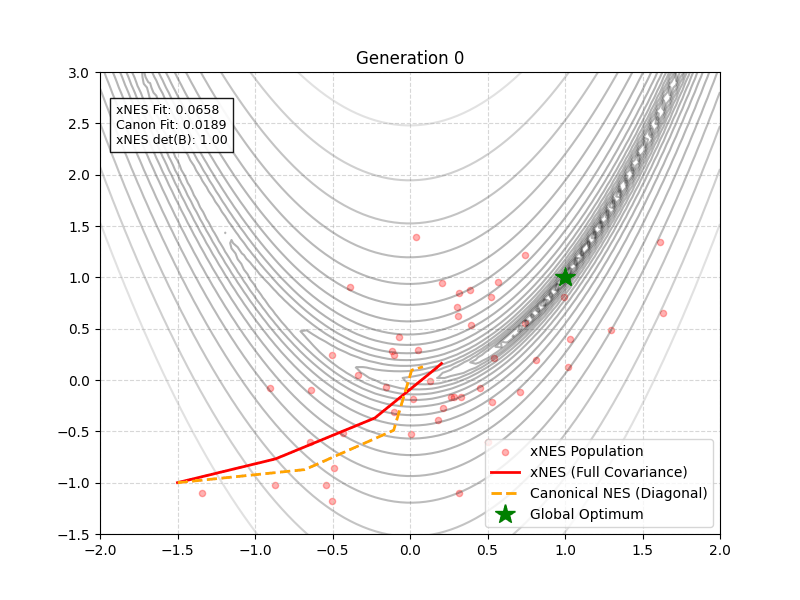
\includegraphics[width=0.3\textwidth]{xnesvsnes/frame_00_delay-0.33s.png}
		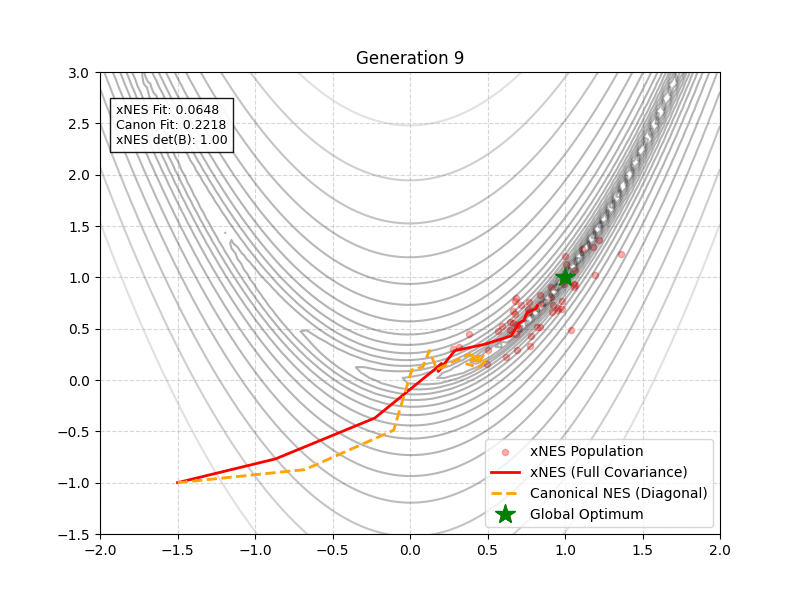
\includegraphics[width=0.3\textwidth]{xnesvsnes/frame_09_delay-0.33s.png}
		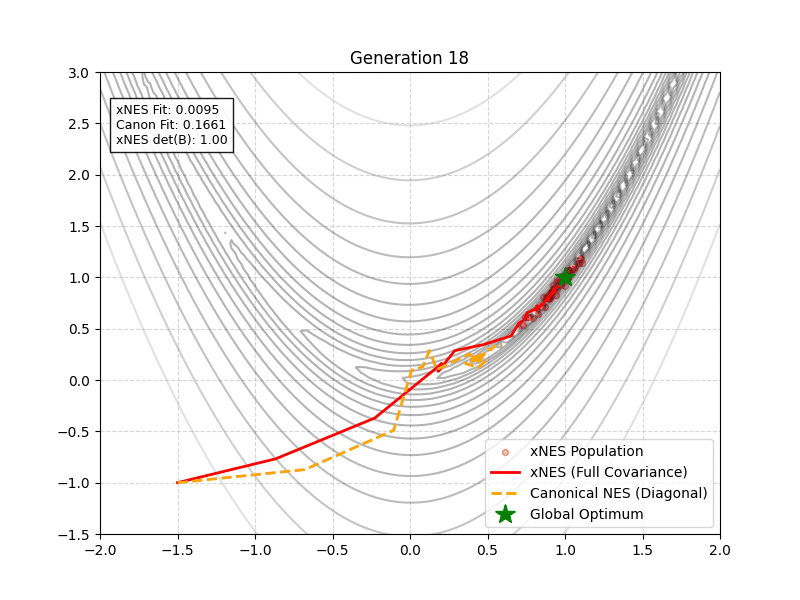
\includegraphics[width=0.3\textwidth]{xnesvsnes/frame_18_delay-0.33s.png}
		
		\vspace{0.3cm}
		
		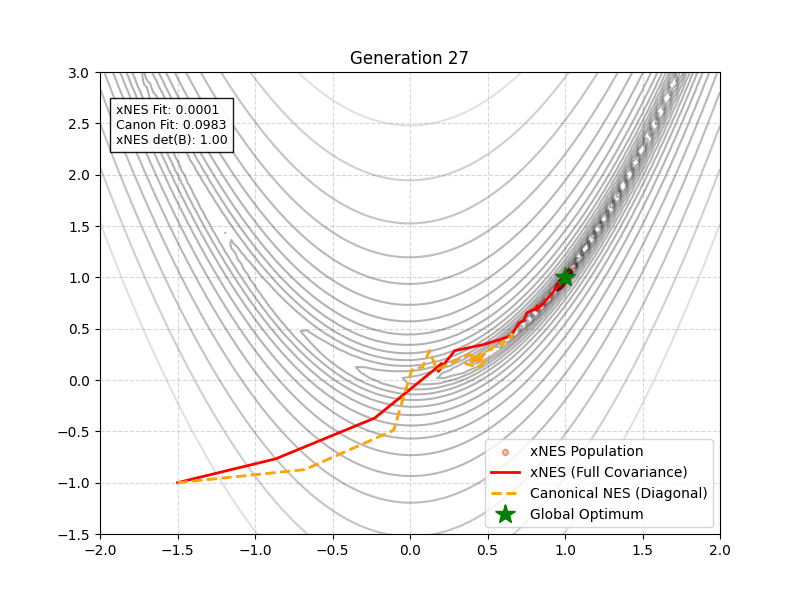
\includegraphics[width=0.3\textwidth]{xnesvsnes/frame_27_delay-0.33s.png}
		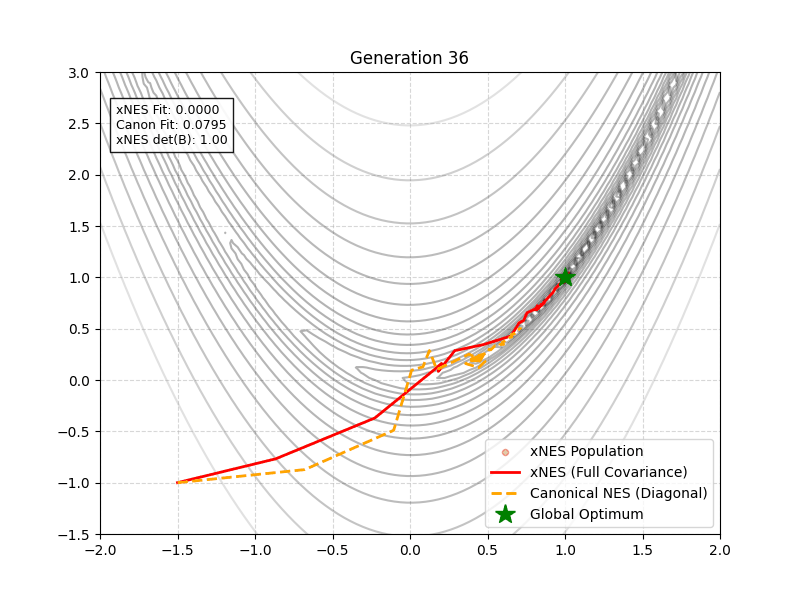
\includegraphics[width=0.3\textwidth]{xnesvsnes/frame_36_delay-0.33s.png}
		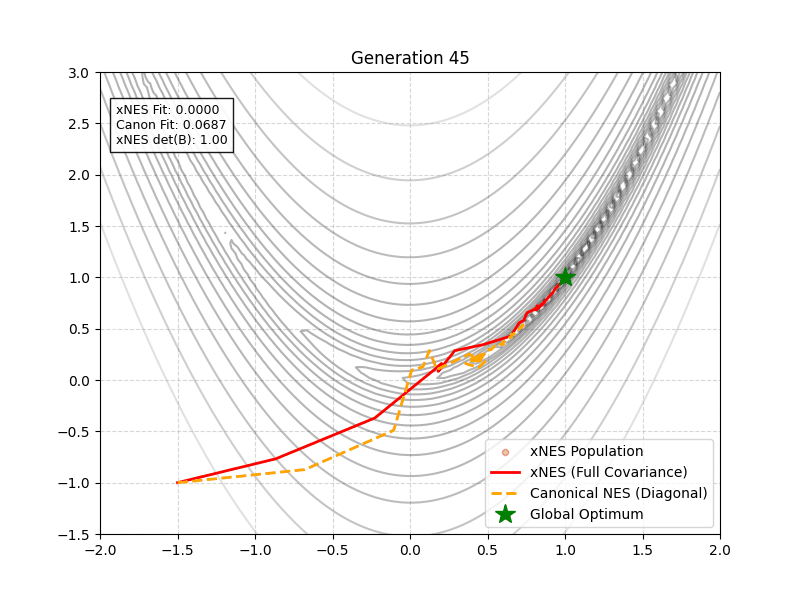
\includegraphics[width=0.3\textwidth]{xnesvsnes/frame_45_delay-0.33s.png}
		
		\vspace{0.3cm}
		
		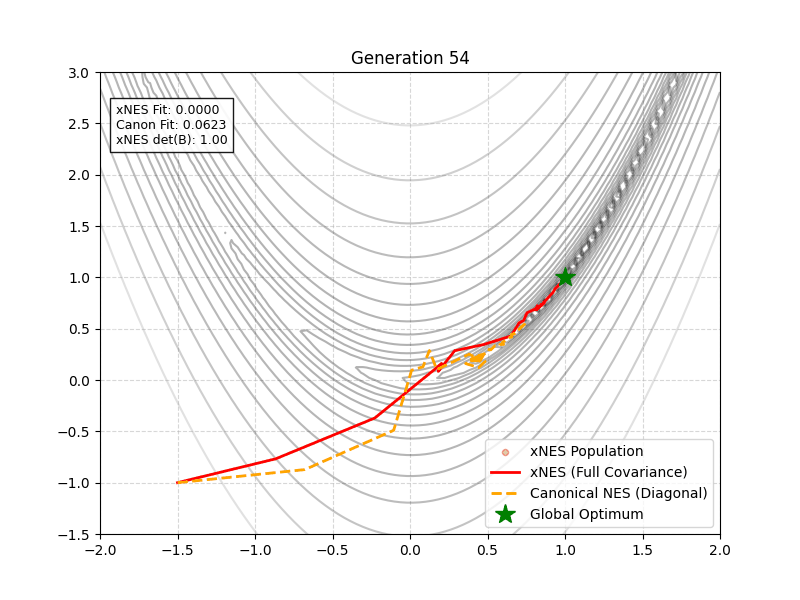
\includegraphics[width=0.3\textwidth]{xnesvsnes/frame_54_delay-0.33s.png}
		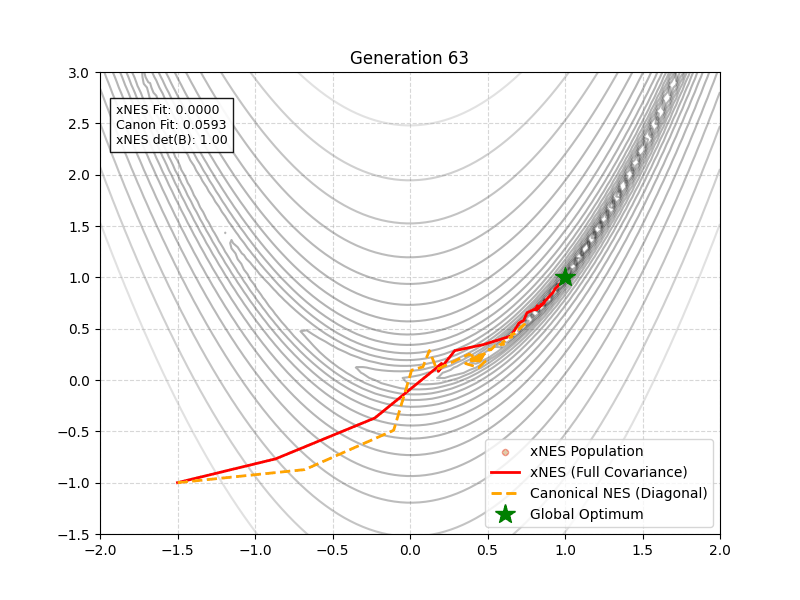
\includegraphics[width=0.3\textwidth]{xnesvsnes/frame_63_delay-0.33s.png}
		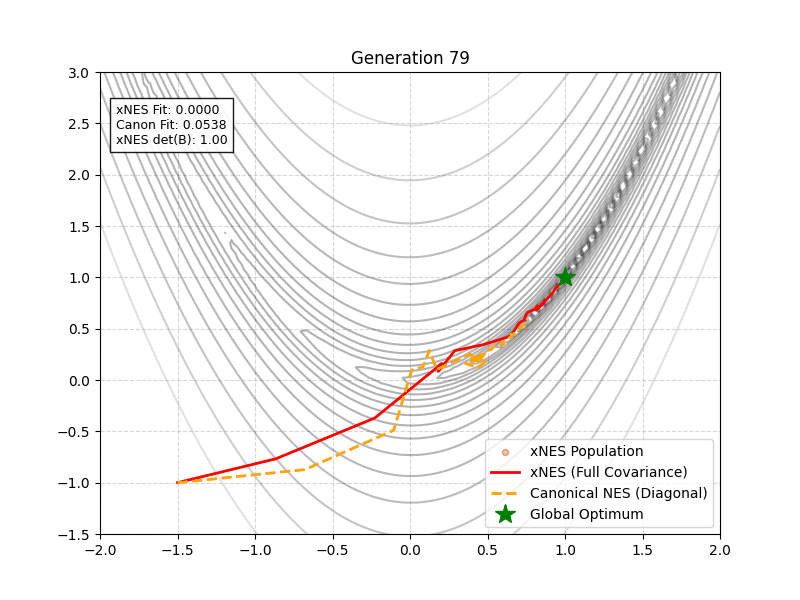
\includegraphics[width=0.3\textwidth]{xnesvsnes/frame_79_delay-0.33s.png}
		
		\caption{Sự khác nhau giữa xNES và Canonical NES}
		\label{fig:xnes_evolution}
	\end{figure}
	% ================================================================
	
	\section{Thực nghiệm}
	
	Thuật toán được kiểm nghiệm trên hàm Rastrigin hai chiều:
	\[
	f(x) = 10d + \sum_{i=1}^d (x_i^2 - 10\cos 2\pi x_i).
	\]
	
	\begin{figure}[H]
		\centering
		
		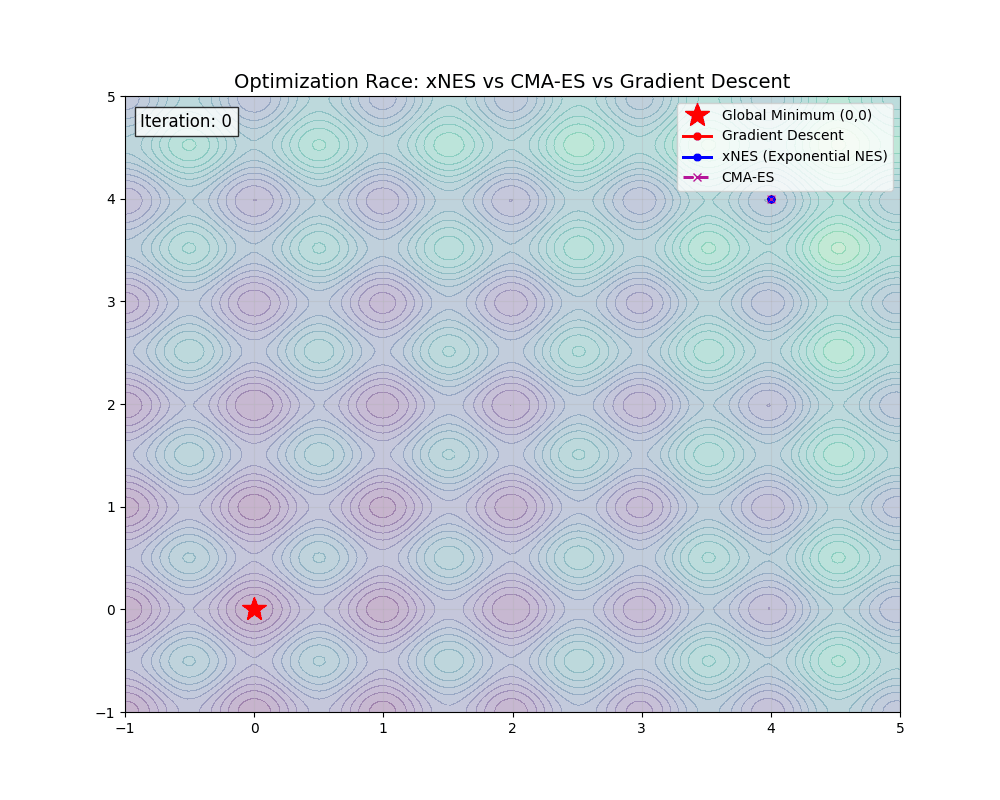
\includegraphics[width=0.4\textwidth]{xnes/frame_00_delay-0.2s.png}
		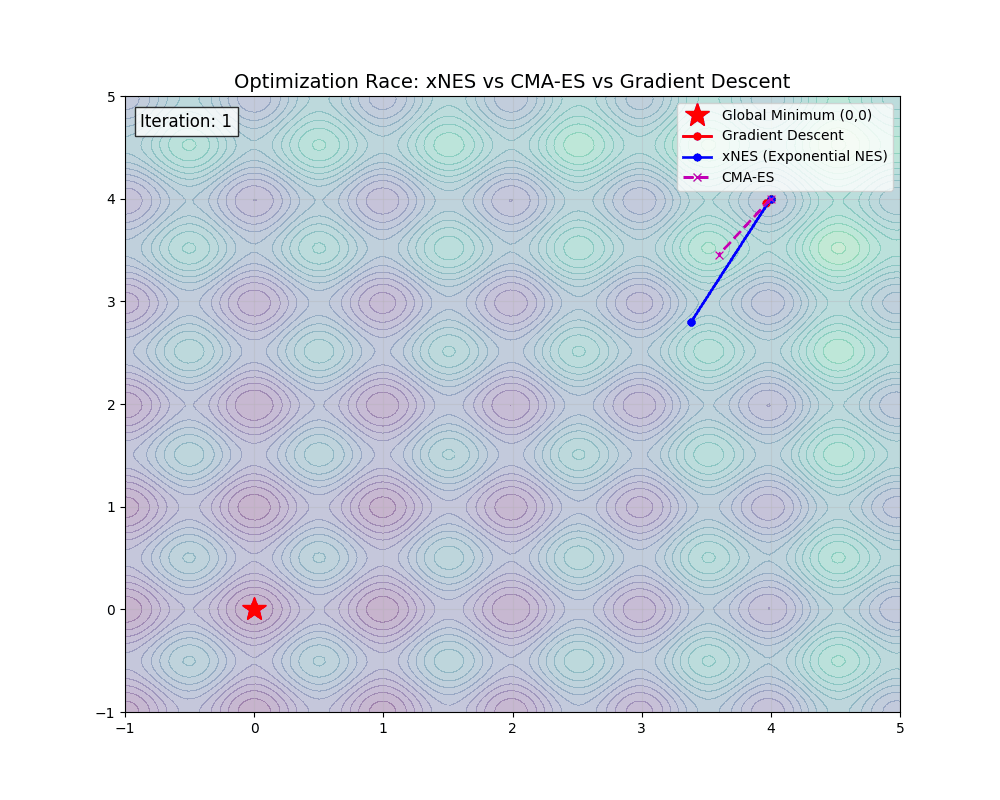
\includegraphics[width=0.4\textwidth]{xnes/frame_01_delay-0.2s.png}
		\vspace{0.1cm}
		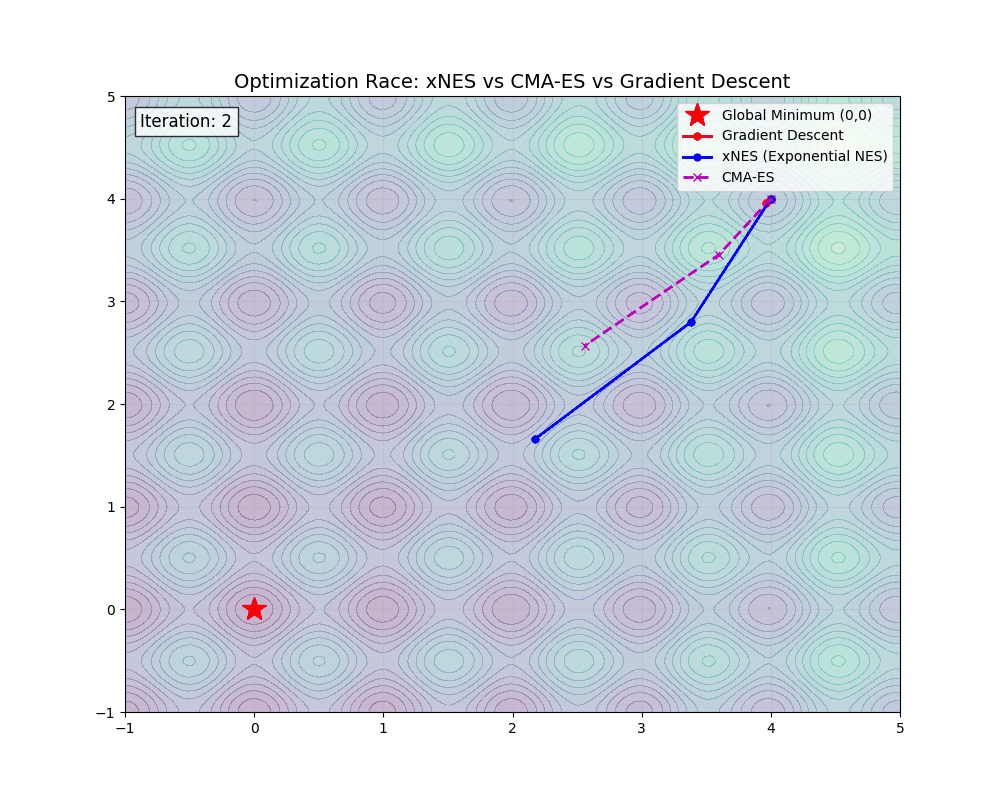
\includegraphics[width=0.4\textwidth]{xnes/frame_02_delay-0.2s.png}
		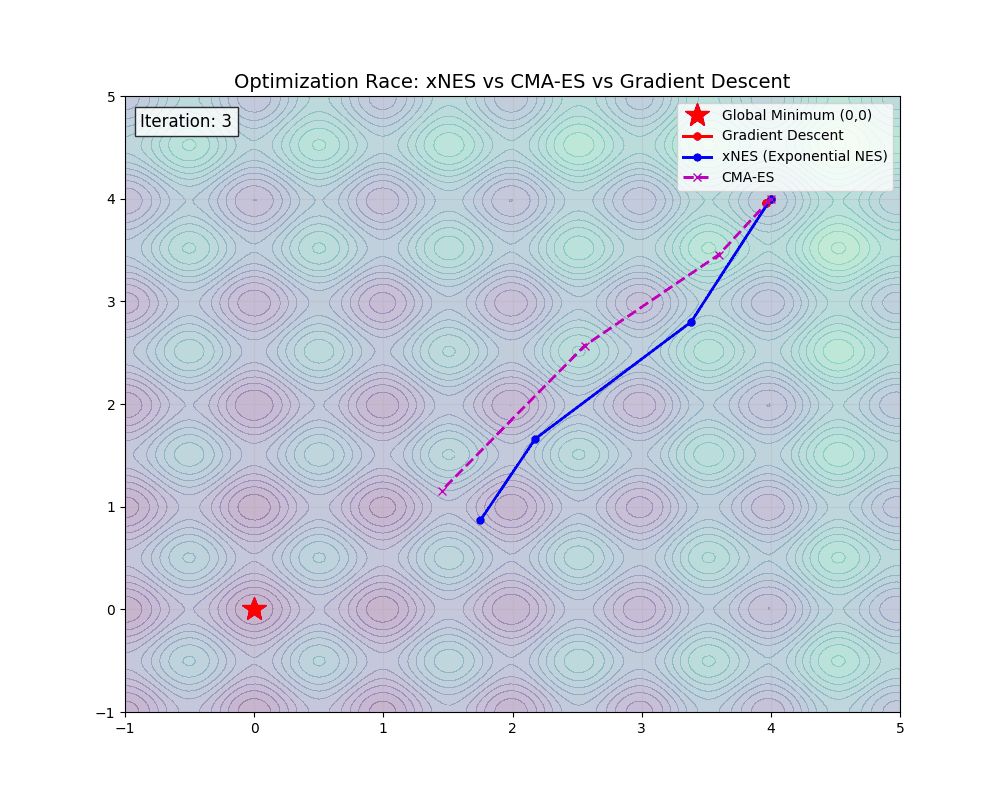
\includegraphics[width=0.4\textwidth]{xnes/frame_03_delay-0.2s.png}
		\vspace{0.1cm}
		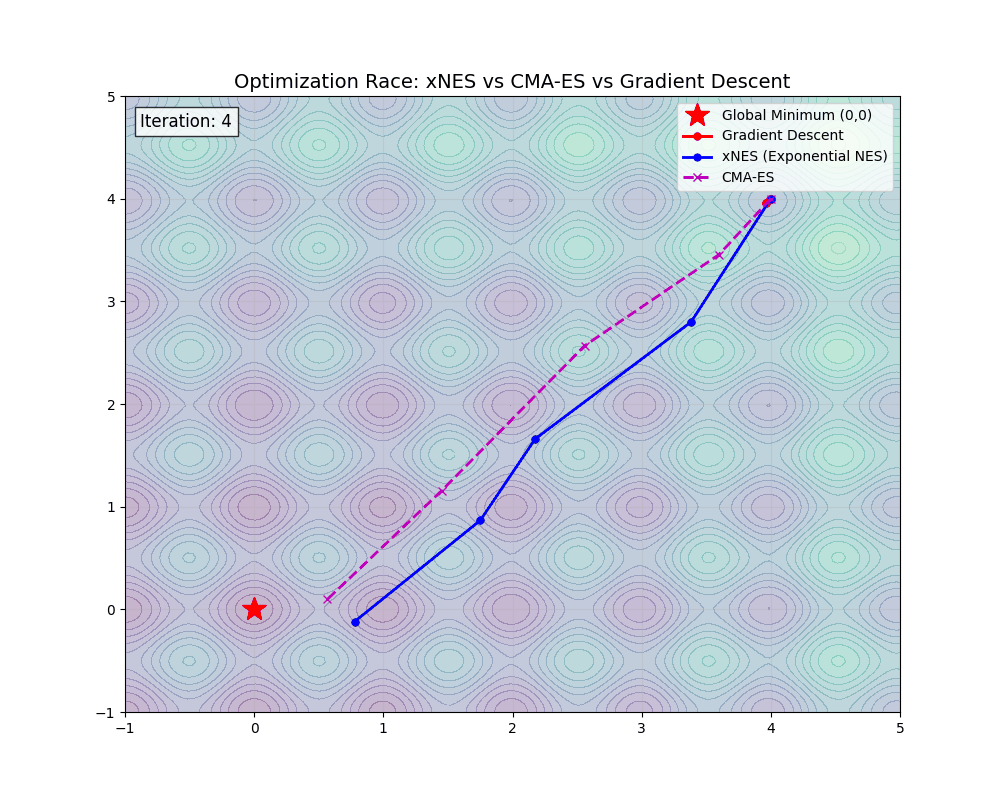
\includegraphics[width=0.4\textwidth]{xnes/frame_04_delay-0.2s.png}
		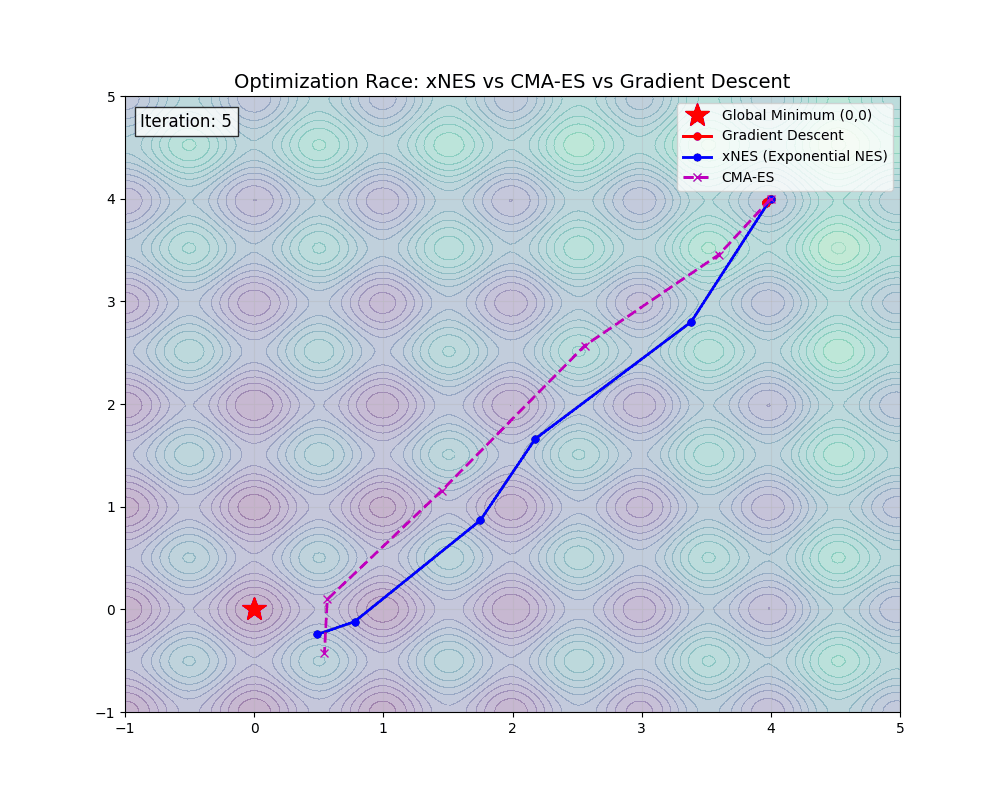
\includegraphics[width=0.4\textwidth]{xnes/frame_05_delay-0.2s.png}
		\vspace{0.1cm}
		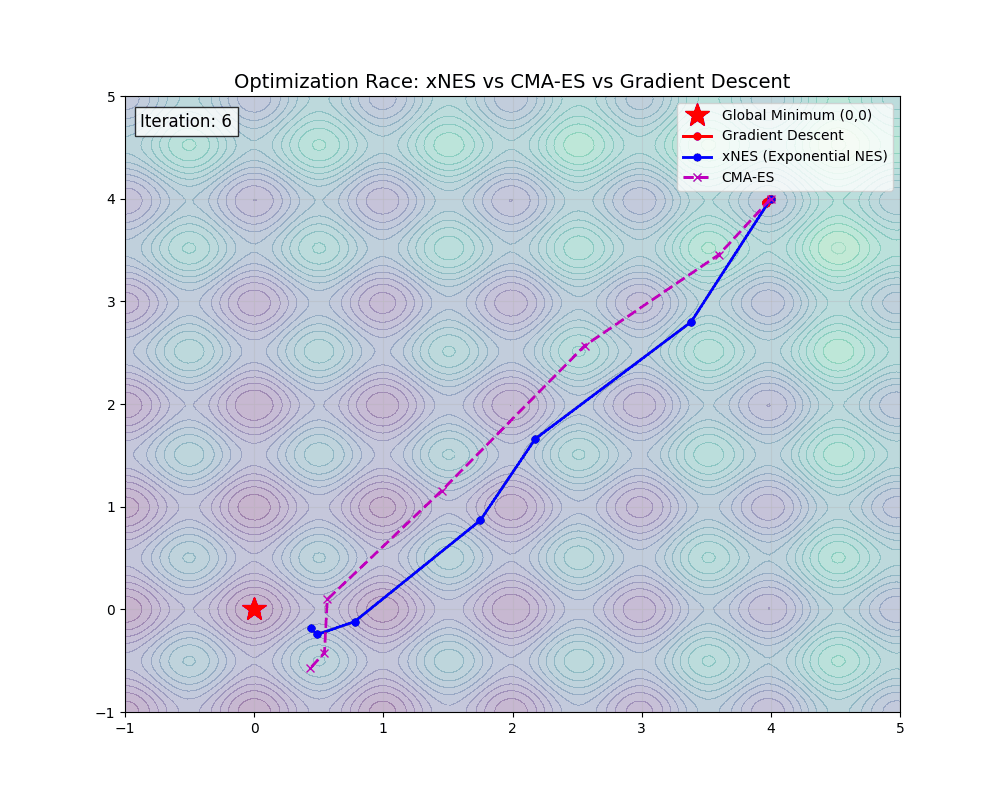
\includegraphics[width=0.4\textwidth]{xnes/frame_06_delay-0.2s.png}
		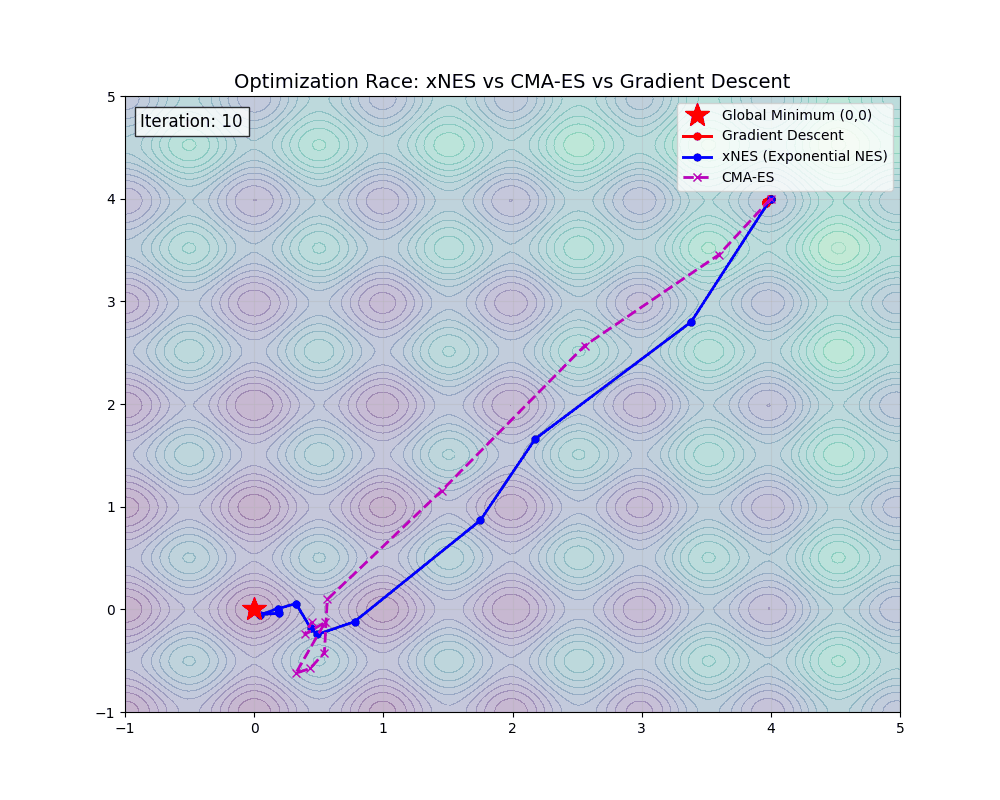
\includegraphics[width=0.4\textwidth]{xnes/frame_10_delay-0.2s.png}
		\vspace{0.1cm}
		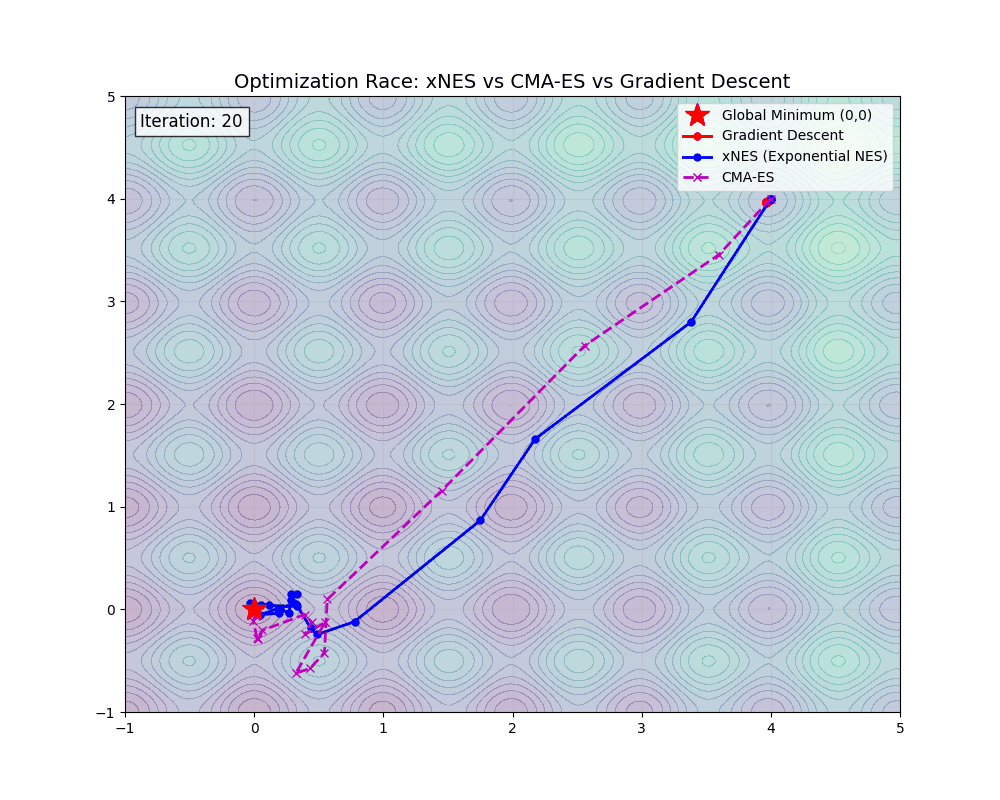
\includegraphics[width=0.4\textwidth]{xnes/frame_20_delay-0.2s.png}
		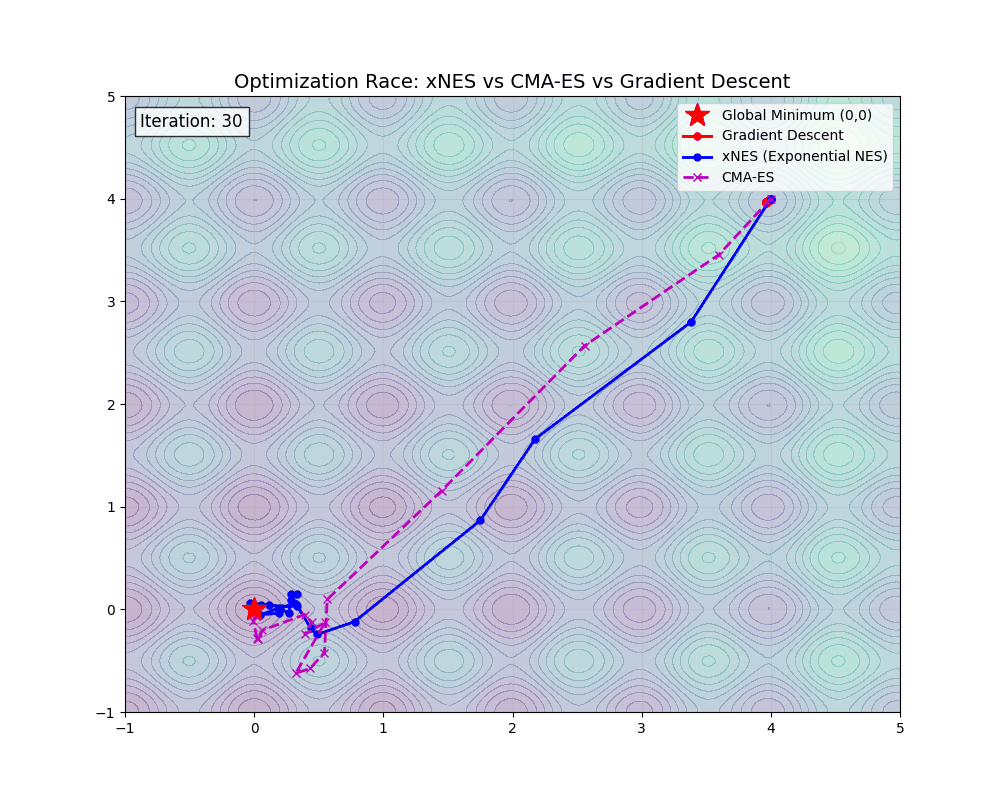
\includegraphics[width=0.4\textwidth]{xnes/frame_30_delay-0.2s.png}
		\caption{xNES | CMA-ES | Gradient Descent }
		\label{fig:xnesvsother}
	\end{figure}
	
	Kết quả cho thấy xNES, CMA-ES hội tụ ổn định về nghiệm toàn cục trong khi phương pháp gradient thường thất bại khi $\sigma$ nhỏ.
	
	% =========================================================
	\section{Kết luận}
	Báo cáo đã trình bày khung lý thuyết của Natural Evolution Strategies và biến thể xNES. Kết quả thực nghiệm cho thấy xNES đạt hiệu năng cao, ổn định và có nền tảng toán học rõ ràng, trở thành một lựa chọn hiệu quả cho các bài toán tối ưu hóa hộp đen.
	
\end{document}
